\documentclass{article}

\usepackage{subcaption,tikz,pgfplots,pgfplotstable,filecontents}

\pgfplotsset{compat=newest,table/search path={../../../../data/figures}}
\usepgfplotslibrary{groupplots,fillbetween}

\tikzset{
    png export/.style={
        external/system call/.add=
            {}
            {; convert -density 300 -transparent white "\image.pdf" "\image.png"; mv \image.png png;},
        %
        },
    }



\usetikzlibrary{external}
\tikzexternalize[prefix=pdf/]
\tikzset{png export}

\begin{document}

\tikzsetnextfilename{diagram-BsrCartoon}
\begin{figure}
    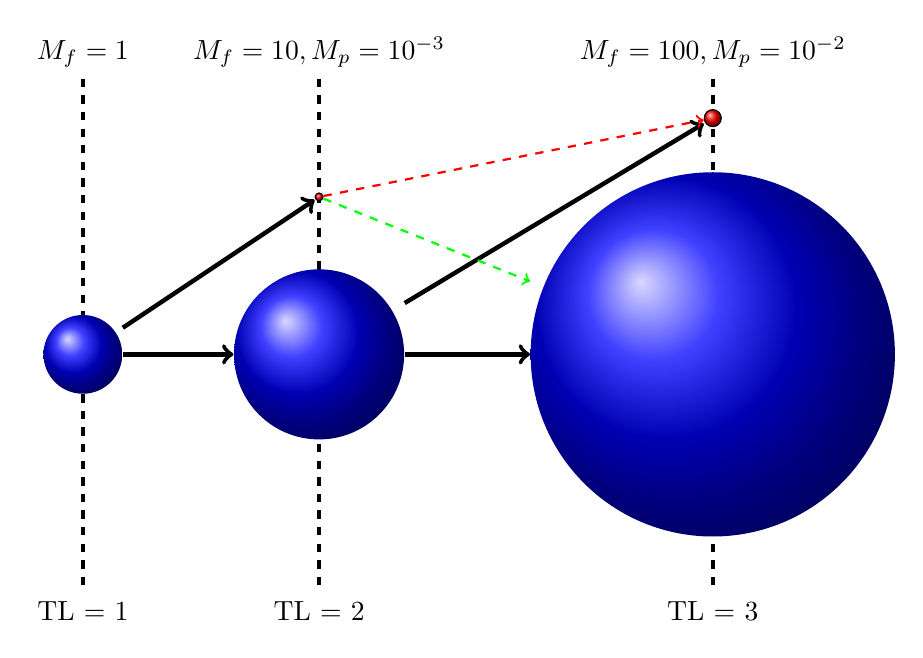
\begin{tikzpicture}
        \node [inner sep = .05cm] (p1) at (3,1) {};
        \node [inner sep = .108cm] (p2) at (8,2) {};
        \node [inner sep = .5cm] (s1) at (0,-1) {};
        \node [inner sep = 1.08cm] (s2) at (3,-1) {};
        \node [inner sep = 2.313cm] (s3) at (8,-1) {};
        \draw[->,ultra thick] (s1) -> (s2);
        \draw[->,ultra thick] (s2) -> (s3);
        \draw [ultra thick, dashed] (8,2.5) node [anchor = south]  {$M_f = 100,M_p=10^{-2}$}--(8,-4) node [anchor = north] {TL = 3};
        \draw [ultra thick, dashed] (3,2.5) node [anchor = south]  {$M_f = 10,M_p=10^{-3}$}--(3,-4) node [anchor = north] {TL = 2};
        \draw [ultra thick, dashed] (0,2.5) node [anchor = south]  {$M_f = 1$}--(0,-4) node [anchor = north] {TL = 1};
        \draw[->,ultra thick] (s1) -> (p1);
        \draw[->,ultra thick] (s2) -> (p2);
        \draw[->,dashed,thick,red] (p1) -> (p2);
        \draw[->,dashed,thick,green] (p1) -> (s3);
        \shade [ball color=blue] (s1) circle (.5cm);
        \shade [ball color=blue] (s2) circle (1.08cm);
        \shade [ball color=blue] (s3) circle (2.313cm);
        \draw [ball color=red] (p1) circle (.05cm);
        \draw [ball color = red] (p2) circle (.108cm);
    \end{tikzpicture}
\end{figure}

\tikzsetnextfilename{diagram-Cartoon}
\begin{figure}
    \begin{tabular}{c c}
        a. Null Model& b. Refuge\\
        \includegraphics[width=2in]{extra/Null.png}&
        \includegraphics[width=2in]{extra/Null+Ref.png}\\
        c. Concomittant& d. Refuge and Concomittant\\
        \includegraphics[width=2in]{extra/Null+Con.png}&
        \includegraphics[width=2in]{extra/Con+Ref.png}\\
    \end{tabular}
\end{figure}

\tikzsetnextfilename{diagram-ConcomittantPredation}
\begin{figure}
    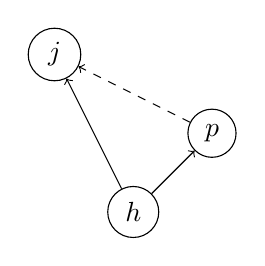
\begin{tikzpicture}
        \node[draw,circle] at (0,0) (j) {$j$};
        \node[draw,circle] at (1,-2) (h) {$h$};
        \node[draw,circle] at (2,-1) (p) {$p$};
        \draw[->] (h)--(j);
        \draw[->] (h)--(p);
        \draw[->,dashed] (p)--(j);
    \end{tikzpicture}
\end{figure}

\tikzsetnextfilename{diagram-NicheModel}
\begin{figure}
    \begin{tikzpicture}
        \draw (0,0)--(10,0)
        node[anchor = west] {$n$};
        \draw (0,.2)--(0,-.2)
        node[anchor = north] {$0$};
        \draw (10,.2)--(10,-.2)
        node[anchor = north] {$1$};
        %Predator
        \fill (7,0) circle (.07) 
        node[anchor = north]  {$n_j$};
        %Predator Diet
        \draw (7,0)--(7,.75)--(2,.75)--(2,.5);
        \draw (.3,0) -- (.3,.5) -- (3.7,.5) -- (3.7,0);
        \draw[dashed] (2,.5) -- (2,0) 
        node[anchor = south east] {$c_j$};
        \draw[<->] (.3,-.5) -- (3.7,-.5)
        node[fill=white,pos = 0.5] {$r_j$}; 
        \draw[dashed] (.3,0)--(.3,-.55);
        \draw[dashed] (3.7,0)--(3.7,-.55);
        %Prey
        \fill (3,0) circle (.07) 
        node[anchor = north west]  {$n_i$};
        \draw(4.2,-2) circle (.3)
        node {$i$};
        \draw[->] (4.5,-2) -- (5.5,-2);
        \draw(5.8,-2) circle (.3)
        node {$j$};
    \end{tikzpicture}
\end{figure}

\tikzsetnextfilename{diagram-Models}
\begin{figure}
    \begin{tikzpicture}
        \node (null) at (0,0) {\includegraphics[width=.45\textwidth]{extra/Null.png}};
        \node[inner sep = 0pt,text width =.5\linewidth,align=center,anchor=south] (nullTitle) at (null.north) {\subcaption[]{Null}};
        \node[anchor = west] (ref) at (null.east) {\includegraphics[width=.45\textwidth]{extra/Null+Ref.png}};
        \node[inner sep = 0pt,text width =.5\linewidth,align=center,anchor=south] (refTitle) at (ref.north) {\subcaption[]{Host Refuge}};
        \node[inner sep = 0pt,text width =.5\linewidth,align=center,anchor=north] (conTitle) at (null.south) {\subcaption[]{Concomittant}};
        \node[inner sep = 0pt,text width =.5\linewidth,align=center,anchor=north] (fullTitle) at (ref.south) {\subcaption[]{Full}};
        \node[anchor = north] (con) at (conTitle.south) {\includegraphics[width=.45\textwidth]{extra/Null+Con.png}};
        \node[anchor = north] (full) at (fullTitle.south) {\includegraphics[width=.45\textwidth]{extra/Con+Ref.png}};
    \end{tikzpicture}
\end{figure}
%\node [inner sep = 0pt,text width =.5\linewidth,align=center,anchor=south] at (leg4b.north) {\subcaption[]{$Z_p = 10^{-4}$\label{fig:frac-bio-h}}};
 
\end{document}
